% MDPI-style working supplementary package; generated from frozen Markdown at Git ad00fb0.
\documentclass[notspecified,supfile,submit,moreauthors]{Definitions/mdpi}

\makeatletter
\gdef\@pubvolume{0}
\gdef\@issuenum{0}
\gdef\@articlenumber{0}
\gdef\@pubyear{}
\gdef\@copyrightyear{}
\makeatother
\firstpage{1}
\datereceived{}
\daterevised{}
\dateaccepted{}
\datepublished{}
\setlength{\headheight}{20pt}
\fancyfoot[R]{}

% Final title and keywords confirmed by the author on 2026-10-20.
% Author identities, order, and affiliations were supplied by the author and
% updated on 2026-10-20. Corresponding authors: Vassiliy Serbin and Aray Kassenkhan.
\newcommand{\PaperTitle}{Profile Poisoning and Selective-Update Bias in Online Behavioral Biometric Authentication}
\newcommand{\orcidauthorA}{0009-0006-2621-0454}
\newcommand{\orcidauthorB}{0000-0002-5807-3873}
\newcommand{\orcidauthorC}{0000-0002-6355-9544}
\newcommand{\orcidauthorD}{0000-0003-1042-1530}
\newcommand{\orcidauthorE}{0000-0003-0716-5265}
\newcommand{\orcidauthorF}{0009-0002-4089-9332}
\newcommand{\orcidauthorG}{0009-0009-8985-5892}
\newcommand{\PaperAuthors}{Madi Gali $^{1}$\orcidA{}, Vassiliy Serbin $^{2,*}$\orcidB{}, Aray Kassenkhan $^{3,*}$\orcidC{}, Aliya Turegeldinova $^{4}$\orcidD{}, Bakytzhan Amralinova $^{5}$\orcidE{}, Shyndauyl Nugumanov $^{5}$\orcidF{} and Yersain Chinibayev $^{3}$\orcidG{}}
\newcommand{\PaperAuthorNames}{Madi Gali, Vassiliy Serbin, Aray Kassenkhan, Aliya Turegeldinova, Bakytzhan Amralinova, Shyndauyl Nugumanov and Yersain Chinibayev}
\newcommand{\PaperAffiliations}{%
$^{1}$ \quad Department of Cybersecurity, Institute of Automation and Information Technologies, Satbayev University, Almaty 050013, Kazakhstan; \href{mailto:gali.m@stud.satbayev.university}{gali.m@stud.satbayev.university}\\
$^{2}$ \quad Department of Information Systems, Institute of Automation and Information Technologies, Satbayev University, Almaty 050013, Kazakhstan; \href{mailto:v.serbin@satbayev.university}{v.serbin@satbayev.university}\\
$^{3}$ \quad Department of Software Engineering, Institute of Automation and Information Technologies, Satbayev University, Almaty 050013, Kazakhstan; \href{mailto:a.kassenkhan@satbayev.university}{a.kassenkhan@satbayev.university} (A.K.); \href{mailto:y.chinibayev@satbayev.university}{y.chinibayev@satbayev.university} (Y.C.)\\
$^{4}$ \quad Department of Management and Mathematical Economics, Satbayev University, Almaty, Kazakhstan; \href{mailto:a.turegeldinova@satbayev.university}{a.turegeldinova@satbayev.university}\\
$^{5}$ \quad Project Management Institute, Satbayev University, Almaty, Kazakhstan; \href{mailto:b.amralinova@satbayev.university}{b.amralinova@satbayev.university} (B.A.); \href{mailto:s.nugumanov@satbayev.university}{s.nugumanov@satbayev.university} (S.N.)
}
\newcommand{\PaperCorrespondence}{Correspondence: \href{mailto:v.serbin@satbayev.university}{v.serbin@satbayev.university} (V.S.); \href{mailto:a.kassenkhan@satbayev.university}{a.kassenkhan@satbayev.university} (A.K.)}
\newcommand{\PaperKeywords}{behavioral biometrics; continuous authentication; template update; online adaptation; profile poisoning; selective-update bias; mobile security; adversarial machine learning}
\newcommand{\PaperAbstract}{Behavioral continuous authentication can update a user's profile during operation, but accepted-only adaptation links access errors to future model state. Prior biometric work established separate authentication and update thresholds and quantified erroneous impostor inclusion and genuine-update misses. We examine their coupled security and adaptation consequences in score-level mobile authentication using frozen HMOG long short-term memory scores, a synthetic feature-space shift, and an independent two-day McGill Gait protocol. Poisoning samples were separated from future impostor probes. The strongest benchmark assumed access to claimant scores and presented up to eight initially accepted samples ranked near the authentication boundary; reconnaissance and candidate screening were not counted. At the reference operating points, Blind exponential moving-average (EMA) updating increased post-poison attack success rate from 22.92\% to 53.96\% on HMOG and from 12.37\% to 32.09\% on McGill. An enrollment-anchored Guarded EMA condition kept the reference-point result close to Frozen. This direction did not persist across recalibrated policies. Under the nominal-1\% calibration condition, the mean Blind-minus-Frozen effect was negative on both datasets for the tested boundary strategy. On the same HMOG conditional cohort, Blind EMA reduced attack success by 0.447 percentage points but increased false rejection by 6.89 points and half total error rate by 3.22 points. Full-cohort false rejection at this strict condition was 80.79\% on HMOG and 90.25\% on McGill. The Guarded rule added no update margin when the current authentication threshold reached or exceeded the enrollment mean. In separate temporal evaluations, Guarded did not improve late genuine acceptance relative to Frozen. A label-aware, non-deployable Oracle-all diagnostic changed profile trajectories and reduced false rejection, but increased false acceptance. The results show that poisoning effects, genuine rejection, update-gate activity, calibration transfer, and attack feasibility depend on the operating point and should be evaluated together.}

\Title{\PaperTitle}
\Author{\PaperAuthors}
\AuthorNames{\PaperAuthorNames}
\address{\PaperAffiliations}
\corres{\PaperCorrespondence}
\abstract{Supplementary methods and results for the accompanying working manuscript.}
\keyword{\PaperKeywords}

\renewcommand{\thefigure}{S\arabic{figure}}
\renewcommand{\thetable}{S\arabic{table}}
\providecommand{\theHfigure}{}
\providecommand{\theHtable}{}
\renewcommand{\theHfigure}{supp.figure.\arabic{figure}}
\renewcommand{\theHtable}{supp.table.\arabic{table}}

\begin{document}

\section*{Supplementary Methods}\phantomsection\label{sm:overview}

\subsection*{S1. Experimental chronology and evidence status}\phantomsection\label{sm:s1}

The branches used the evidential roles below. ``Primary reporting contrast'' identifies manuscript focus and does not retroactively make sequential HMOG development confirmatory.

\begin{table}[H]
\begin{adjustwidth}{-\extralength}{0cm}
\footnotesize
\setlength{\tabcolsep}{3pt}
\renewcommand{\arraystretch}{1.14}
\begin{tabularx}{\fulllength}{L l L L L}
\toprule
\textbf{Stage} & \textbf{Dataset} & \textbf{Parameter and data status} & \textbf{Role} & \textbf{Outer outcomes accessed?} \\
\midrule
Previous accepted-only baseline & HMOG & Inherited EMA and frozen score pipeline & Defines Blind EMA and the open update pathway & Previously evaluated \\
Attack v2 & HMOG & Fixed attack protocol developed on HMOG & Exploratory mechanism evidence & Yes \\
Guarded lambda sweep & HMOG & Exploratory outer-data sweep; \(\lambda=0.25\) carried forward & Update-authorization intervention & Yes \\
Clean temporal analysis & HMOG & Frozen synthetic shift protocol & Exploratory mechanism analysis & Yes \\
Oracle-all & HMOG & Label-aware fixed diagnostic & Genuine-evidence availability intervention & Yes \\
TQ-EMA v1 & HMOG & Validation-selected under branch-specific rule & Supporting outer evaluation & Yes \\
TQ-EMA v2 & HMOG & Validation gate failed & Validation-stopped & No \\
Adaptive Quantile Profile & HMOG & Validation gate failed & Validation-stopped & No \\
Cross-day replication & McGill & \(\lambda=0.25\) transferred before Day 2 & Directional mechanism corroboration & Yes, after viability gate \\
Operating-point sensitivity & HMOG and McGill & Fixed scores, \(\alpha\), \(\lambda\), pools, and seeds & Prospectively specified sensitivity on previously inspected caches & Existing caches reused \\
\bottomrule
\end{tabularx}
\end{adjustwidth}
\end{table}

The method sequence matters. HMOG attack and Guarded results were developed on already inspected outer caches. The McGill transfer fixed the HMOG reporting rule before Day-2 scores were loaded. The operating-point analysis was specified after reference outcomes had been inspected and therefore remains a sensitivity analysis rather than untouched confirmation.

\subsection*{S2. HMOG preprocessing and score generation}\phantomsection\label{sm:s2}

The primary pipeline used 100 enrolled HMOG subjects in closed-set verification. The nominal design contained 24 sessions per subject. The retained data comprised 2,392 usable sessions and 4,784 sequences after documented missing or empty files. The physical accelerometer and gyroscope \(x,y,z\) axes were read; metadata and session identifiers were excluded from the model input. Accelerometer and gyroscope rows were paired by acquisition order after truncation to the shorter file, without timestamp resampling. The experiment assumed the nominal 100 Hz sampling rate and did not estimate the realized rate.

For each usable session, the pipeline discarded the first 500 samples and retained the next 20 non-overlapping 100-sample windows. Mean, standard deviation, minimum, maximum, root mean square, and skewness were calculated for six channels, yielding 36 features per window. Ten adjacent windows formed one \(10\times36\) sequence. The sequence step was ten windows, so the two retained sequences did not overlap or cross session boundaries. The previous study states that the 20-window retention cap equalized session contributions and bounded computation. It does not document why the initial 500 samples were discarded, nor establish that either choice is optimal or free from early-session sampling bias.

Five outer folds used \(g(r)=(r-1)\bmod5\). For fold \(f\), group \(f\) was test, group \((f+1)\bmod5\) was validation/calibration, and the other three groups were model fitting. All subjects occurred in each partition through separate sessions. A StandardScaler was fitted to flattened fitting-partition time steps and applied unchanged to validation and test data.

The LSTM accepted \(10\times36\) inputs. It contained two recurrent layers with 64 hidden units each, layer normalization, a 32-unit ReLU layer, dropout 0.30, and a 100-class softmax. Training used cross-entropy, Adam with learning rate \(10^{-3}\), batch size 256, at most 20 epochs, and early-stopping patience 4. The canonical code also used \texttt{ReduceLROnPlateau} with factor 0.5 and patience 2. The claimant score was the corresponding softmax probability. A separate Paper 3 cache-generation run executed this canonical procedure, trained one fold-specific LSTM per fold, and saved its checkpoint, scaler, validation scores, and drift-specific test scores. The resulting caches were then held fixed and hash-identified across the method comparisons; the attack and adaptation runners did not retrain the LSTM. This was protocol-matched regeneration, not verified byte-identical reuse of the weights or score predictions reported in the previous study. The cache-generation metadata did not preserve a Git revision, a hash of the cache-builder source or input sequence archive, or the complete package environment, so that earlier generation invocation is not cryptographically closed even though downstream frozen manifests identify the exact resulting cache files.

The clean temporal replay ordered sessions by recorded numeric identifier and sequences by within-session position. Public fold numbers 1--5 corresponded to internal zero-based indices 0--4 and drift seeds 42--46. For each fold, the canonical transform sampled one vector \(z\sim\mathcal{N}(0,I_{36})\) and used \(v=z/(\lVert v\rVert_2+10^{-12})\). The same fold direction was used for every subject and for \(D=1\) and \(D=2\). For subject-specific chronological sequence rank \(j=0,\ldots,n-1\), every one of the ten time steps received the same displacement

\[
\Delta X_j=D\frac{j}{n-1}v.
\]

The rank covered all original standardized test sequences. The replay selected \texttt{within=0} as adaptation and \texttt{within=10} as checkpoint only after drift scores had been cached; the ramp was not reconstructed over adaptation candidates alone. The global scenario used the selected-\(D\) cache for claimant and impostor scores. The claimant-only scenario combined selected-\(D\) genuine scores with \(D=0\) impostor scores. The source confirms this executed order but does not independently establish that numeric session identifiers encode a validated natural behavioral chronology.

Across the five test positions, 500 victim-fold paths contained 2,392 complete source session pairs: 394 paths had five pairs, 104 had four, and two had three. Requiring at least four retained 498 paths and 2,386 adaptation-checkpoint pairs; the two excluded test paths were subject 57 in public folds 4 and 5. The early and late endpoints each contained 996 unique genuine checkpoints. Counts are observation inventories, not independent inferential units. The hash-matched canonical injection source is retained, while the authoritative temporal manifest records the executed runner hash without retaining byte-identical runner source; this limits cryptographic reconstruction of that invocation.

\subsection*{S3. Calibration, threat model, and attack implementation}\phantomsection\label{sm:s3}

\subsubsection*{S3.1. Reference and sensitivity calibration}\phantomsection\label{sm:s3-1}

HMOG validation genuine scores initialized the profile moments. For each claimant, genuine validation scores were labelled positive and all other validation identities supplied pooled negative observations, with every observation entering once and no source-identity reweighting. The executed canonical implementation called \texttt{\seqsplit{sklearn.metrics.roc\_curve}} with \texttt{drop\_intermediate=False}, computed \(\mathrm{FNR}=1-\mathrm{TPR}\), and selected the first returned ROC index minimizing \(|\mathrm{FPR}-\mathrm{FNR}|\) through \texttt{np.nanargmin}. Its returned threshold was used without interpolation, and the descriptive approximate EER was \((\mathrm{FPR}+\mathrm{FNR})/2\) at that same index. The claimant score was the corresponding softmax probability, so larger values were more genuine-like. Finally, \(k=(\mu_0-\tau_0)/\sigma_0\) reproduced the selected threshold. This documents the executed approximate-EER rule rather than an exact or interpolated EER. The Paper 2 release records scikit-learn 1.7.2, but the separate Paper 3 cache-generation metadata does not preserve a complete package environment, so that version is not asserted for the generation invocation.

McGill reference thresholds minimized pooled Day-1 HTER per claimant, with exact ties resolved toward the higher threshold. Sensitivity calibration used the following recorded float64 rule on each dataset. For nominal target \(\beta\), candidate thresholds were the reference threshold and \texttt{nextafter(v,+infinity)} for every unique calibration-impostor score \(v\). Candidates had to be finite and no lower than reference. The smallest candidate satisfying \(\operatorname{mean}(I\geq\tau)\leq\beta\) was selected; reference was retained if it already met the constraint. The operational rule \texttt{score\ \textgreater{}=\ threshold} placed tied scores together. Test and Day-2 outcomes did not enter calibration.

The sensitivity procedure kept \(\mu_0\) and the second moment fixed and recomputed claimant-specific \(k\) for each \(\tau_0\). Negative \(k\) values were retained. EMA \(\alpha=0.05\), Guarded \(\lambda=0.25\), and the canonical sigma-floor behavior were fixed.

\subsubsection*{S3.2. Attacker capabilities}\phantomsection\label{sm:s3-2}

\begin{table}[H]
\begin{adjustwidth}{-\extralength}{0cm}
\footnotesize
\setlength{\tabcolsep}{3pt}
\renewcommand{\arraystretch}{1.14}
\begin{tabularx}{\fulllength}{L L L L}
\toprule
\textbf{Capability or assumption} & \textbf{Boundary strategy} & \textbf{Random strategy} & \textbf{Scope} \\
\midrule
Access decision observable & Yes & Yes & An attempt is associated with an access outcome \\
Claimant score available & Assumed for ranking & Not required & Boundary results require score access or equivalent ordering information \\
Candidate pool & Preassigned held-out test impostor pool & Same pool type & Real acquisition of a complete pool is not modeled \\
Selection & Initially accepted samples ranked by smallest non-negative margin & Uniform order without replacement & Boundary is the stronger benchmark \\
Screening charged to \(K\) & No & No separate screening & \(K=8\) is not an eight-query attack \\
Binary-feedback search demonstrated & No & Ranking not required & Practical score-free boundary search remains untested \\
Model internals or gradients & Not used & Not used & Score-informed does not by itself imply model white-box access \\
Dataset identity labels & Used offline to define claimant, impostor, poison, and probe sets & Same & Not exposed to Blind or Guarded online updating; Oracle controls are explicitly label-aware \\
Replay, sensor injection, OS compromise & Excluded & Excluded & Results concern the online profile-update surface \\
\bottomrule
\end{tabularx}
\end{adjustwidth}
\end{table}

For HMOG, whole source-identity/session groups were assigned to poison or probe pools before candidate selection. Groups did not cross pools, but source identities were not necessarily disjoint. Maximum sequences were sampled once, and budgets \(K\in\{0,1,2,4,8\}\) were nested prefixes. The primary reference cohort required eight initially accepted boundary candidates. It contained 49,889 of 50,000 fold-victim-repeat paths; 111 paths were excluded. The historical random and \(K=0\) summaries used this same common reference cohort.

For operating-point sensitivity, random summaries used all 50,000 structurally valid HMOG paths and all 2,000 McGill paths. Each boundary condition used its own common \(K=8\)-feasible cohort. HMOG eligibility was 49,889, 49,753, and 9,088 paths at reference, nominal 5\%, and nominal 1\%; corresponding victim-fold counts were 500, 500, and 302. McGill eligibility was 1,456, 1,369, and 1,001 paths across 18, 18, and 17 victims. Infeasible paths were exclusions, not zero-ASR outcomes.

\subsubsection*{S3.3. Local canonical EMA boundary transition}\phantomsection\label{sm:s3-3}

For one permitted canonical update, let \(d=s_t-\mu_t\). From

\[
\mu_{t+1}=(1-\alpha)\mu_t+\alpha s_t,
\qquad
q_{t+1}=(1-\alpha)q_t+\alpha s_t^2,
\]

expansion of \(q_{t+1}-\mu_{t+1}^2\) gives

\[
\sigma_{t+1}^2=(1-\alpha)\left(\sigma_t^2+\alpha d^2\right).
\]

For an observation exactly at the current raw boundary, \(s_t=\mu_t-k\sigma_t\), this becomes

\[
\sigma_{t+1}^2=(1-\alpha)\sigma_t^2(1+\alpha k^2),
\]

and, with fixed \(k\),

\[
\Delta\tau
=k\sigma_t\left[(1-\alpha)-\sqrt{(1-\alpha)(1+\alpha k^2)}\right].
\]

The result assumes \(0<\alpha<1\), \(\sigma_t>0\), a permitted update, an admissible score, and inactive sigma-floor and threshold-clipping branches both before and after the transition. Under those assumptions the bracket is negative, so \(\Delta\tau<0\) for \(k>0\), \(\Delta\tau>0\) for \(k<0\), and \(\Delta\tau=0\) for \(k=0\). This presubmission derivation is explanatory rather than a new empirical result. Attack candidates were selected near the initial boundary, later candidates need not lie on the current boundary, margins were nonzero, Guarded could deny updates, and operating-point cohorts changed. The identity therefore does not by itself determine the sign of a multi-update mean ASR effect.

\subsection*{S4. Endpoints, uncertainty, and reproducibility}\phantomsection\label{sm:s4}

Post-poison ASR was held-out impostor acceptance after the state was frozen. FRR used held-out genuine observations evaluated at that frozen state, and \(\mathrm{HTER}=(\mathrm{ASR}+\mathrm{FRR})/2\). MUR divided incorporated malicious observations by presented malicious observations. The poisoning-experiment GUR replay used a copy of the post-poison state, so it measured update availability and could not change ASR, FRR, or HTER already recorded.

The historical HMOG reference contrast averaged repeats within victim and fold, then folds within each victim. A 10,000-draw paired percentile bootstrap with seed 4242 resampled the 100 victim effects. Its Blind-minus-Frozen estimate was +31.037638 points with CI {[}+26.946230, +35.202592{]}. The sensitivity package used the same paths, estimand, hierarchy, and number of draws but key-derived random streams from master seed 20261004. Its reference CI was {[}+26.966964, +35.106318{]}. Victim effects matched to floating-point tolerance; the interval difference reflects Monte Carlo resampling.

The historical McGill reference package used 1,456 paths across 18 victims and a deterministic stream derived from master seed 20261003, producing {[}+5.579173, +37.344069{]} for the +19.721769-point effect. The sensitivity package used master seed 20261004 and produced {[}+5.498731, +37.240872{]} for the same effect and cohort. Historical sections retain historical CIs, while the sensitivity table uses its own retained intervals consistently.

Clean HMOG outcomes were averaged within subject across available folds before 10,000-draw paired percentile bootstrap. The TQ-v1 primary available-fold analysis contained 100 victims, and a 99-subject complete-five-fold analysis checked its decision. McGill repeats were averaged within subject before paired bootstrap. Five overlapping HMOG fitting partitions and Monte Carlo repeats were not treated as independent inferential units. Within the poisoning operating-point analysis, a secondary product-weight victim-by-impostor-source bootstrap was retained only for HMOG nominal 1\%, boundary \(K=8\): Blind-minus-Frozen was -0.447 points {[}\ensuremath{-}0.515, \ensuremath{-}0.383{]}, and Guarded-minus-Blind was -0.009 {[}\ensuremath{-}0.022, \ensuremath{-}0.001{]}. This analysis covered 100 victims, 9,088 paths, and 100 observed impostor sources; source-resolved outcomes were unavailable for the historical reference poisoning package. Separately, the TQ-v1 clean-temporal late-FAR sensitivity resampled 100 victims and 100 impostor sources over 9,900 observed victim-source pairs; its TQ-v1-minus-Frozen estimate was -1.939 points {[}\ensuremath{-}2.476, \ensuremath{-}1.420{]}. Neither analysis covers training uncertainty or a deployment population, and the poisoning analysis does not cover other operating points or McGill.

The frozen method, McGill, and operating-point packages are identified by tags \texttt{\seqsplit{paper3-method-freeze-2026-10-02}}, \texttt{\seqsplit{paper3-external-mcgill-v1-2026-10-03}}, and \texttt{\seqsplit{paper3-operating-point-sensitivity-v1-2026-10-04}}. The authoritative package registry is:

\begin{table}[H]
\begin{adjustwidth}{-\extralength}{0cm}
\footnotesize
\setlength{\tabcolsep}{3pt}
\renewcommand{\arraystretch}{1.14}
\begin{tabularx}{\fulllength}{L L L}
\toprule
\textbf{Package} & \textbf{Repository-relative manifest} & \textbf{Recorded revision or status} \\
\midrule
Final HMOG method analysis & \path{results/paper3_final_analysis_20261002_v2/manifest.json} & Git \texttt{\seqsplit{476cf9104d5598f88a187d72ef1686f27fcea7cd}}; complete \\
McGill replication & \path{results/paper3_external_mcgill_20261003_v1/manifest.json} & Git \texttt{\seqsplit{1c0eeb8fb9dbbc1113d9aa0faa48cee07c72cce9}}; complete; outer data loaded after the viability gate \\
Operating-point sensitivity & \path{results/paper3_operating_point_sensitivity_20261004_v1/manifest.json} & Git \texttt{\seqsplit{517746fbe6e89268a603fceebefe558409eabb33}}; complete \\
TQ-v1 & \path{results/paper3_tq_clean_drift_20261001_v1/manifest.json} & Complete; source and cache hashes recorded, Git revision absent \\
TQ-v2 & \path{results/paper3_tq_v2_validation_failed_20261001/manifest.json} & Validation failed; source and cache hashes recorded; outer outcomes not loaded \\
Adaptive Quantile & \path{results/paper3_quantile_validation_failed_20261001_v1/manifest.json} & Validation failed; \texttt{outer\_test\_loaded=false} \\
\bottomrule
\end{tabularx}
\end{adjustwidth}
\end{table}

The manifests retain full source/cache or protocol hashes, environment fields, seeds, exclusions, generated-file registries, and status fields according to package scope. The HMOG base-cache schema stores validation scores and labels, clean test inputs and labels, session and within-session indices, and subject names; the drift-cache schema stores test scores and labels, session and within-session indices, drift magnitude, and drift seed, with model checkpoints and scalers retained separately. The operating-point package additionally declares one row per planned path in \texttt{eligibility\_by\_path.csv}, one method outcome per dataset/condition/path/strategy/budget in \texttt{\seqsplit{outcomes\_by\_path.parquet}}, and nominal-1\% HMOG boundary-\(K=8\) source counts in \texttt{\seqsplit{probe\_outcomes\_by\_source.parquet}}. The McGill archive SHA-256 is \texttt{\seqsplit{0e2da09c2d10fb5658c79d362e9e043a2f2822715723238b30cbebd2e7b425d9}}; the locked score-cache hash is \texttt{\seqsplit{3f390ab19fbea15582fbb5a646cf7e631b77b744ab101e97d83edb533717a79b}}.

The operating-point manifest records an initial source hash and a later figure-only action. The current runner hash matches \texttt{post\_run\_actions{[}0{]}.source\_sha256}; the action removed lines between operating-point-specific cohorts and regenerated artwork from frozen tables without recomputing outcomes. All generated-artifact and protocol hashes matched their manifest entries. Recorded protocol checks covered no-update behavior, malicious-update-blocking Oracle/Frozen equivalence in malicious-only streams, nested budgets, split disjointness, update gating, bounded transitions, enrollment anchors, recovery isolation, and deterministic analysis.

\subsection*{S5. McGill classifier and protocol}\phantomsection\label{sm:s5}

The official McGill archive supplied timestamped recordings from subjects \texttt{w001} to \texttt{w020} on two days. Magnetometer, orientation, and temperature channels were excluded. The executed reader selected the supplied fields \texttt{accel\_x}, \texttt{accel\_y}, \texttt{accel\_z}, and \texttt{accel\_mag}; it did not recompute the fourth channel. The archive documentation defines \texttt{accel\_mag} as \(\sqrt{x^2+y^2+z^2}-9.8066\), with acceleration fields in \(\mathrm{m/s^2}\). Median sample interval was 40 ms, approximately 25 Hz. No interpolation was applied. Inputs were non-overlapping 128-sample windows, approximately 5.12 s, with shape \(128\times4\).

One pooled per-channel z-score transform was fitted over all time samples in Day-1 training windows using population standard deviations; any value below \(10^{-8}\) would have been replaced by 1.0. The frozen transform was applied to enrollment and Day 2. Within each subject, Day-1 windows were split chronologically into 60\% fitting, 20\% early-stopping validation, and 20\% enrollment/calibration using floor-valued cut points. Recorded Day-1 counts were 2,840 fitting, 948 validation, and 958 enrollment/calibration windows across 20 subjects. The classifier was a one-layer unidirectional LSTM with input size 4, hidden size 64, final-hidden-state classification, and a 20-class linear head. Training used class-weighted cross-entropy, Adam with learning rate 0.001 and weight decay 0.0001, batch size 128, at most 30 epochs, and validation-loss early stopping with patience 5.

The profile used \(\alpha=0.05\), sigma \(\max(\sqrt{\max(q-\mu^2,0)},10^{-4})\), and the \emph{unclipped} authentication threshold \(\tau=\mu-k\sigma\). Day-1 enrollment genuine scores set \(\mu_0\) and \(q_0\); the threshold minimizing pooled Day-1 HTER set \(\tau_0\), with exact ties resolved toward the higher threshold; and \(k=(\mu_0-\tau_0)/\sigma_0\). Access used \texttt{score >= threshold}. Guarded \(\lambda=0.25\) transferred from HMOG without a McGill sweep or Day-2 tuning, but HMOG's zero lower clamp on the authentication threshold did not transfer. The executed protocol did not record this difference as a planned intervention. Poisoning used 100 repeats, nested \(K\), and an identity-disjoint poison/probe split as close to 50/50 as possible. Boundary reference \(K=8\) retained 1,456 paths across 18 victims; random retained all 2,000 paths. Profiles were frozen before probe and genuine evaluation.

The temporal protocol selected 160 approximately equally spaced Day-2 windows per subject and formed 80 pairs, each containing an adaptation observation followed by an evaluation-only checkpoint. The first and last 20 pairs defined early and late endpoints. All 20 subjects contributed exactly 80 units, for 1,600 unique adaptation candidates and 1,600 unique genuine checkpoints; early and late each contained 400 checkpoints. For each unit, authentication and update eligibility used the pre-update threshold, a permitted adaptation update was applied, and the disjoint checkpoint was then evaluated. Saved \texttt{mean}, \texttt{sigma}, and \texttt{threshold} fields therefore describe the post-adaptation state used for that checkpoint. Matched impostor checkpoints did not update state.

Before any Day-2 score was loaded, the run stopped if training was non-finite, fewer than 16 classes appeared in validation, top-1 validation accuracy was below 20\%, or protocol checks and a synthetic smoke run failed. The fixed classifier achieved 58.12\% validation top-1 accuracy and passed. Day-1/Day-2 separation does not isolate behavioral drift from activity, placement, acquisition, or model-transfer change.

\subsection*{S6. TQ-EMA v1 state and transitions}\phantomsection\label{sm:s6}

TQ-EMA v1 added an isolated recovery route while retaining Guarded \(\lambda=0.25\). Production state contained EMA mean, second moment, derived standard deviation, and authentication threshold. Quarantine state held candidate scores, distinct session identifiers, downward direction, and age. Resetting quarantine did not change production state.

The trusted path used Guarded's effective conjunction. Four observation paths were defined:

\begin{enumerate}
\def\labelenumi{\arabic{enumi}.}
\item
  \(s_t\geq\tau^{\mathrm{update,effective}}_t\): access granted; bounded EMA proposal considered.
\item
  \(\tau^{\mathrm{auth}}_t\leq s_t<\tau^{\mathrm{update,effective}}_t\): access granted; no production update.
\item
  \(\tau^{\mathrm{auth}}_t-b\leq s_t<\tau^{\mathrm{auth}}_t\): access denied; observation enters quarantine only.
\item
  \(s_t<\tau^{\mathrm{auth}}_t-b\): access denied; observation discarded; quarantine reset.
\end{enumerate}

Recovery required \(m\) consecutive candidates from distinct sessions, each below the production mean recorded at the start of the run, with batch range at most \(r\). An intervening non-candidate reset the run. A confirmed batch used its median score for a joint first- and second-moment proposal. Standard deviation and threshold were recomputed from those moments. Proposals had to satisfy

\[
|\Delta\mu|\leq c_\mu,
\qquad
|\Delta\tau|\leq c_\tau,
\qquad
\tau\geq\tau_{\mathrm{enroll}}-A.
\]

A recovery proposal that did not lower the derived threshold was rejected.

\subsection*{S7. TQ-EMA v1 selection}\phantomsection\label{sm:s7}

The validation grid was

\[
b/\sigma_{\mathrm{enroll}}\in\{0.25,0.50,0.75\},
\quad m\in\{2,3\},
\]

\[
\alpha_{\mathrm{recovery}}\in\{0.025,0.050\},
\quad A/\sigma_{\mathrm{enroll}}\in\{0.10,0.25\}.
\]

Fixed controls were \(r=0.50\sigma_{\mathrm{enroll}}\), \(c_\mu=0.10\sigma_{\mathrm{enroll}}\), \(c_\tau=0.05\sigma_{\mathrm{enroll}}\), trusted \(\lambda=0.25\), and trusted \(\alpha=0.05\). The first two complete validation sessions initialized and calibrated the inner profile; remaining sessions formed the tuning stream. Claimant validation used independently generated \(D=2\) scores, while impostor checkpoints used \(D=0\).

Among configurations with late-FAR change no greater than +1.0 percentage point relative to Frozen, selection maximized late-FRR gain with conservative tie-breaking. Success required a late-FRR-gain CI lower bound above zero, mean late-FAR increase at most +1.0 point, HTER degradation at most +0.5 point, and the same conclusion in the 99-subject complete cohort. The limits were experiment-specific constraints.

\subsection*{S8. TQ-EMA v2 recovery episode}\phantomsection\label{sm:s8}

TQ-EMA v2 changed one controller property. Confirmation of a valid downward batch first applied the same bounded recovery proposal and then entered \texttt{RECOVERY\_DOWN}. The authentication decision-rule form remained unchanged. Because the controller changed update history, later state, thresholds, and decisions could differ from v1. During an episode, the controller previewed each canonical trusted proposal and skipped it if either the profile mean or derived threshold would increase.

An episode lasted for the next three distinct session-level adaptation observations and was refreshed by a new confirmed batch. Resetting quarantine did not end an active episode. The v1 grid, caps, anchor, and trusted parameters were retained. A configuration was feasible only when late-FAR increase was at most +1.0 point and HTER degradation at most +0.5 point. Selection failed closed if any fold had no feasible configuration.

\subsection*{S9. Adaptive Quantile Profile}\phantomsection\label{sm:s9}

The Quantile branch replaced EMA moments with a discrete exponentially weighted empirical distribution. Enrollment observations began with equal weights. For normalized non-negative weights, \(Q_p\) was the smallest observed score whose sorted cumulative weight reached \(p\), without interpolation. The state retained \(q_{20}=Q_{0.20}\) and \(q_{50}=Q_{0.50}\). At enrollment,

\[
c=\frac{q_{50,0}-\tau_0}{q_{50,0}-q_{20,0}},
\qquad
\tau_t=q_{50,t}-c(q_{50,t}-q_{20,t}).
\]

The fixed, unclipped \(c\) reproduced \(\tau_0\) within floating-point tolerance. A path was invalid when \(q_{50,0}-q_{20,0}<10^{-8}\). For an authorized score, existing weights were multiplied by \(\rho\), the new score was appended with weight \(1-\rho\), weights were normalized, and quantiles and threshold were recomputed.

Accepted-only Quantile updated after authentication acceptance. Oracle-all Quantile applied the same access-decision formula to its own current state, then used ground-truth genuineness to make every genuine adaptation candidate update-eligible regardless of that candidate's recorded outcome. It was non-deployable. The only tuned value was \(\rho\in\{0.80,0.90,0.95\}\). Accepted-only Quantile determined feasibility under the +1.0-point FAR and +0.5-point HTER limits; the branch failed closed if any fold had no feasible \(\rho\).

\subsection*{S10. Branch-specific inference}\phantomsection\label{sm:s10}

For TQ-v1, subjects were averaged across available folds before 10,000-draw paired percentile bootstrap. A secondary victim-by-impostor-source bootstrap assessed late FAR, and the 99-subject cohort checked the decision. Trusted and recovery event totals were audit counts rather than independent observations.

TQ-v2 and Quantile summaries are validation decision evidence, not outer inference. Their packages are \texttt{\seqsplit{results/paper3\_tq\_v2\_validation\_failed\_20261001/}} and \texttt{\seqsplit{results/paper3\_quantile\_validation\_failed\_20261001\_v1/}}; TQ-v1 is in \texttt{\seqsplit{results/paper3\_tq\_clean\_drift\_20261001\_v1/}}. Both validation-stopped packages record that outer outcomes were not loaded.

\section*{Supplementary Results}\phantomsection\label{sr:overview}

\subsection*{S1. TQ-EMA v1 outer evaluation}\phantomsection\label{sr:s1}

TQ-EMA v1 reached its permitted outer evaluation in claimant-only HMOG \(D=2\). The primary available-fold subject analysis contained 100 victims. Late FRR/\allowbreak FAR/\allowbreak HTER were 33.43\%/20.92\%/27.18\%, compared with 32.53\%/22.86\%/27.70\% for Frozen. The paired late-FRR gain was -0.90 percentage points (95\% CI {[}-1.80, 0.00{]}), so the recovery criterion was not met. Late FAR changed by -1.94 points (95\% CI {[}-2.46, -1.43{]}), and HTER gain was +0.52 points (95\% CI {[}+0.10, +0.94{]}). A secondary victim-by-impostor-source late-FAR bootstrap gave -1.94 points (95\% CI {[}-2.48, -1.42{]}).

The 99-victim complete-five-fold cohort did not reverse the decision: its late-FRR-gain CI lower bound was -1.92 points. The \(D=2\) audit recorded 1,404 trusted updates and 49 confirmed recovery updates. These totals are not independent observations.

\startlandscape
\begin{table}[H]
\caption{Fold-specific TQ-v1 validation selections. Rows document selection inputs and are not pooled outer estimates. The redundant encoded configuration identifier is omitted because every selected parameter it encoded is shown separately. Subject 57 was excluded from validation folds 3 and 4 because fewer than four complete adaptation-checkpoint session pairs were available. Source: \protect\path{results/paper3_tq_clean_drift_20261001_v1/}.\label{tab:s1}}
\footnotesize
\setlength{\tabcolsep}{3pt}
\renewcommand{\arraystretch}{1.2}
\begin{tabularx}{\textwidth}{c c c c c c c c c}
\toprule
\textbf{Fold} & \textbf{Validation subjects} & \textbf{Band / \(\sigma_{\mathrm{enroll}}\)} & \textbf{Confirmation sessions} & \textbf{Recovery \(\alpha\)} & \textbf{Anchor / \(\sigma_{\mathrm{enroll}}\)} & \textbf{Validation late-FRR gain, pp} & \textbf{Late-FAR change, pp} & \textbf{HTER change, pp} \\
\midrule
1 & 100 & 0.25 & 3 & 0.025 & 0.10 & 0.00 & -0.38 & -0.19 \\
2 & 100 & 0.50 & 2 & 0.025 & 0.10 & -0.50 & -0.29 & +0.10 \\
3 & 99 & 0.25 & 2 & 0.050 & 0.10 & -1.01 & +0.07 & +0.54 \\
4 & 99 & 0.25 & 3 & 0.025 & 0.10 & 0.00 & -1.22 & -0.61 \\
5 & 100 & 0.25 & 2 & 0.025 & 0.10 & -2.00 & +0.08 & +1.04 \\
\bottomrule
\end{tabularx}
\end{table}
\finishlandscape

\subsection*{S2. TQ-EMA v2 validation stopping}\phantomsection\label{sr:s2}

TQ-v2 completed fold-specific validation before any outer score was loaded. Folds 1, 2, 3, and 5 had feasible selections, all with negative late-FRR gains. Fold 4 had no configuration satisfying both the +1.0-point late-FAR limit and +0.5-point HTER-degradation limit.

\begin{table}[H]
\caption{TQ-v2 validation-gate results. Subject 57 was excluded in folds 3 and 4 because fewer than four complete adaptation-checkpoint session pairs were available. Fold 4 triggered the fail-closed rule. Its best unconstrained late-FRR gain was -4.55 points, and the minimum HTER degradation in the grid was +0.89 points. The frozen \texttt{validation\_failure.json} records \texttt{outer\_test\_loaded=false}; no TQ-v2 outer estimate exists. Source: \protect\path{results/paper3_tq_v2_validation_failed_20261001/}.\label{tab:s2}}
\begin{adjustwidth}{-\extralength}{0cm}
\footnotesize
\setlength{\tabcolsep}{3pt}
\renewcommand{\arraystretch}{1.18}
\begin{tabularx}{\fulllength}{c c L C C C C}
\toprule
\textbf{Fold} & \textbf{Validation subjects} & \textbf{Selection status} & \textbf{Selected late-FRR gain, pp} & \textbf{Late-FAR change, pp} & \textbf{HTER change, pp} & \textbf{Feasible configurations} \\
\midrule
1 & 100 & Feasible & -3.50 & -2.61 & +0.44 & 14 \\
2 & 100 & Feasible & -1.50 & -2.12 & -0.31 & 24 \\
3 & 99 & Feasible & -1.01 & -1.19 & -0.09 & 24 \\
4 & 99 & No feasible configuration & -- & -- & -- & 0 \\
5 & 100 & Feasible & -2.50 & -2.28 & +0.11 & 24 \\
\bottomrule
\end{tabularx}
\end{adjustwidth}
\end{table}

\subsection*{S3. Adaptive Quantile validation stopping}\phantomsection\label{sr:s3}

No \(\rho\in\{0.80,0.90,0.95\}\) satisfied the Accepted-only Quantile gate in any fold. The descriptively least-bad unconstrained value was \(\rho=0.95\) in each fold. At that value, across-fold descriptive means for Accepted-only Quantile were late-FRR gain -10.64 points, late-FAR change -4.89 points, and HTER change +2.87 points relative to Frozen. Oracle-all Quantile at the same \(\rho\) had late-FRR gain -4.62, late-FAR change -1.83, and HTER change +1.39 points.

Oracle-all reduced the additional FRR deficit associated with accepted-only eligibility, but neither information regime outperformed Frozen on the validation late-FRR endpoint. Fold denominators were 100, 100, 99, 99, and 100 subjects; subject 57 was excluded in folds 3 and 4 because fewer than four complete adaptation-checkpoint session pairs were available. All folds failed the gate, \texttt{outer\_test\_loaded=false}, and no outer Quantile estimate exists. Source: \texttt{\seqsplit{results/paper3\_quantile\_validation\_failed\_20261001\_v1/}}.

\begin{table}[H]
\caption{Evaluation status of supporting recovery and state probes. Outcomes apply to the frozen implementations and parameter grids and do not reject their broader method families.\label{tab:s3}}
\begin{adjustwidth}{-\extralength}{0cm}
\footnotesize
\setlength{\tabcolsep}{3pt}
\renewcommand{\arraystretch}{1.18}
\begin{tabularx}{\fulllength}{L L L C L}
\toprule
\textbf{Probe} & \textbf{Data stage reached} & \textbf{Gate outcome} & \textbf{Outer estimate} & \textbf{Evaluation status} \\
\midrule
TQ-EMA v1 & Validation and permitted outer evaluation & Late-FRR recovery criterion not met & Yes & Stopped after outer evaluation \\
TQ-EMA v2 & Validation only & Fold 4 had no feasible configuration & No & Fail-closed validation stop \\
Adaptive Quantile Profile & Validation only & No feasible \(\rho\) in any fold & No & Fail-closed validation stop \\
\bottomrule
\end{tabularx}
\end{adjustwidth}
\end{table}

\begin{table}[H]
\caption{Recorded partition and temporal-observation counts. Values come from frozen metadata and output inventories. Counts are not multiplied across methods, drift levels, or scenarios and are not treated as independent inferential units. HMOG nominal session counts are distinguished from the recorded complete-pair inventory.\label{tab:s4}}
\begin{adjustwidth}{-\extralength}{0cm}
\scriptsize
\setlength{\tabcolsep}{3pt}
\renewcommand{\arraystretch}{1.18}
\begin{tabularx}{\fulllength}{L L L L}
\toprule
\textbf{Dataset / partition} & \textbf{Recorded source inventory} & \textbf{Included temporal observations} & \textbf{Recorded temporal exclusions} \\
\midrule
HMOG test replay & 500 victim-fold paths; 2,392 complete session pairs (394\(\times\)5, 104\(\times\)4, 2\(\times\)3) & 498 paths; 2,386 adaptation candidates and 2,386 checkpoints; 996 early and 996 late checkpoints & Subject 57 in public folds 4 and 5 \\
HMOG genuine calibration & 500 claimant-fold profiles; 4,784 genuine scores (394\(\times\)10, 104\(\times\)8, 2\(\times\)6) & 4,770 scores for 498 temporally eligible profiles & Same two test-path exclusions when forming the temporal cohort \\
McGill Day 1 & 4,746 windows across 20 subjects & 2,840 fitting; 948 validation; 958 enrollment/calibration & None at subject level \\
McGill Day 2 temporal & 4,976 source windows; 3,200 selected windows & 1,600 adaptation candidates and 1,600 checkpoints; 400 early and 400 late checkpoints & None; 544 reference boundary attack exclusions are separate \\
\bottomrule
\end{tabularx}
\end{adjustwidth}
\end{table}

\subsection*{S4. Operating-point diagnostics}\phantomsection\label{sr:s4}

The primary paired operating-point effect figure remains in the main article. Three frozen diagnostics remain supplementary because their aggregation units differ from the victim-macro effect table.

\begin{figure}[H]
\begin{adjustwidth}{-\extralength}{0cm}
\centering
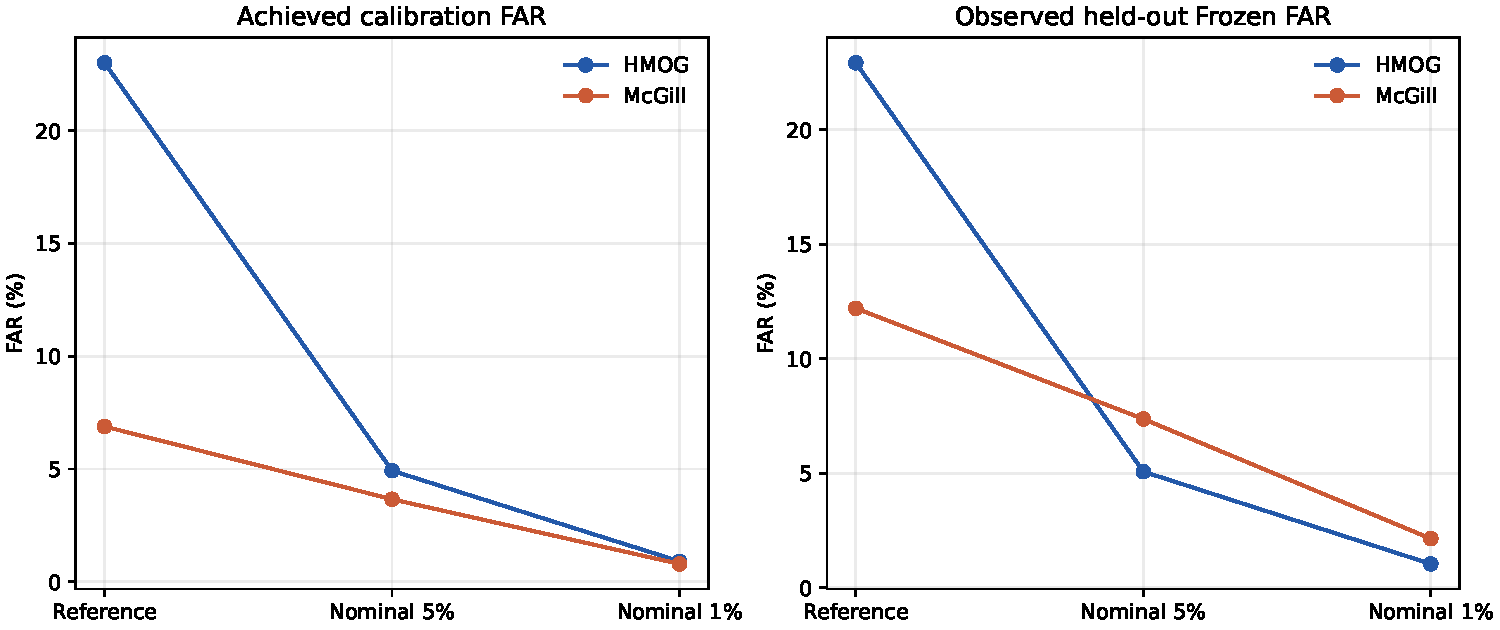
\includegraphics[width=\fulllength,height=0.72\textheight,keepaspectratio]{figures/figureS1_calibration_vs_heldout_far.pdf}
\end{adjustwidth}
\caption{Achieved calibration FAR and full-cohort held-out Frozen FAR at reference, nominal-5\%, and nominal-1\% conditions. Calibration values are unweighted claimant-profile means; held-out values are victim-macro estimates over all structurally valid random-\(K=0\) paths. Source: \protect\path{results/paper3_operating_point_sensitivity_20261004_v1/figures/calibration_vs_heldout_far.pdf}.\label{fig:s1}}
\end{figure}

\begin{figure}[H]
\begin{adjustwidth}{-\extralength}{0cm}
\centering
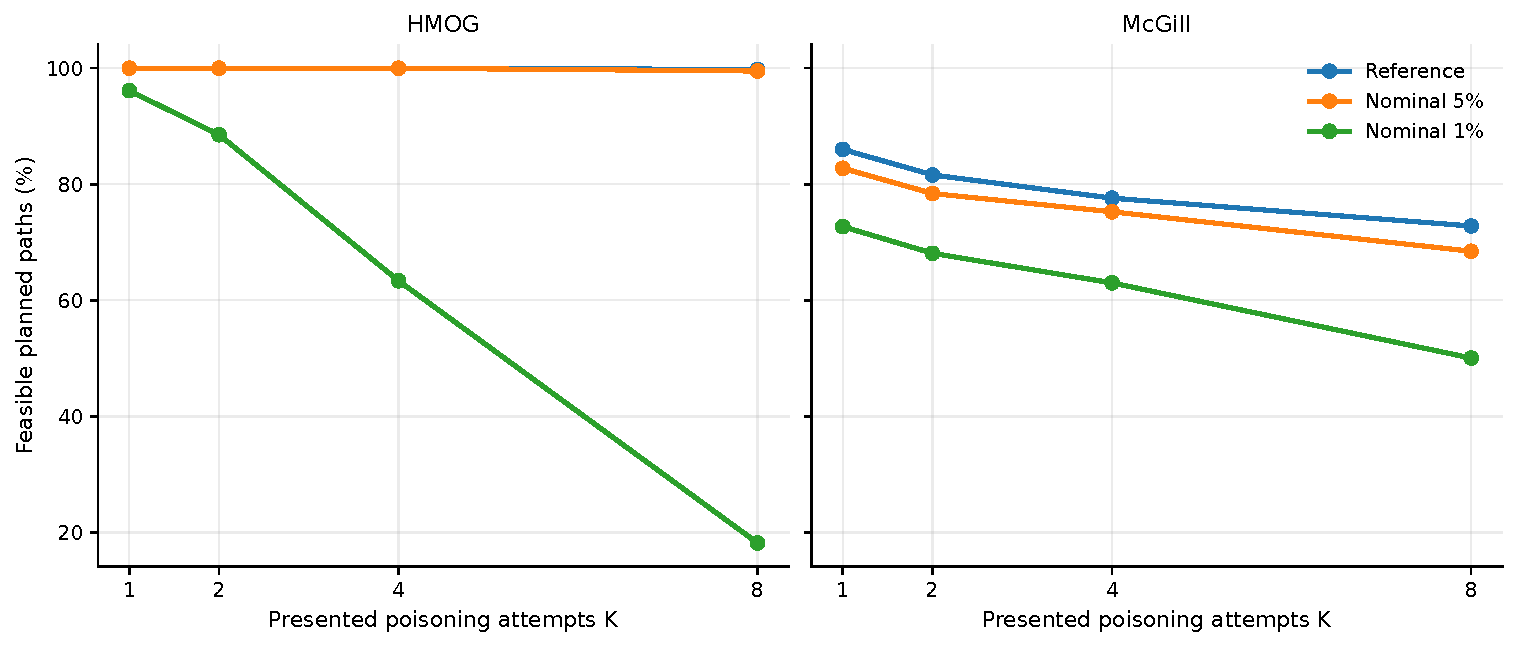
\includegraphics[width=\fulllength,height=0.72\textheight,keepaspectratio]{figures_revision_20261005/figureS2_boundary_feasibility.pdf}
\end{adjustwidth}
\caption{Per-budget boundary feasibility across operating points. Each point is the fraction of all planned paths with at least \(K\) initially accepted candidates for the displayed \(K\). The operating-point effect curves use the common \(K=8\)-feasible cohort within each condition; infeasible paths were excluded rather than assigned zero ASR. Source: \protect\path{results/paper3_operating_point_sensitivity_20261004_v1/eligibility_summary.csv}.\label{fig:s2}}
\end{figure}

\begin{figure}[H]
\begin{adjustwidth}{-\extralength}{0cm}
\centering
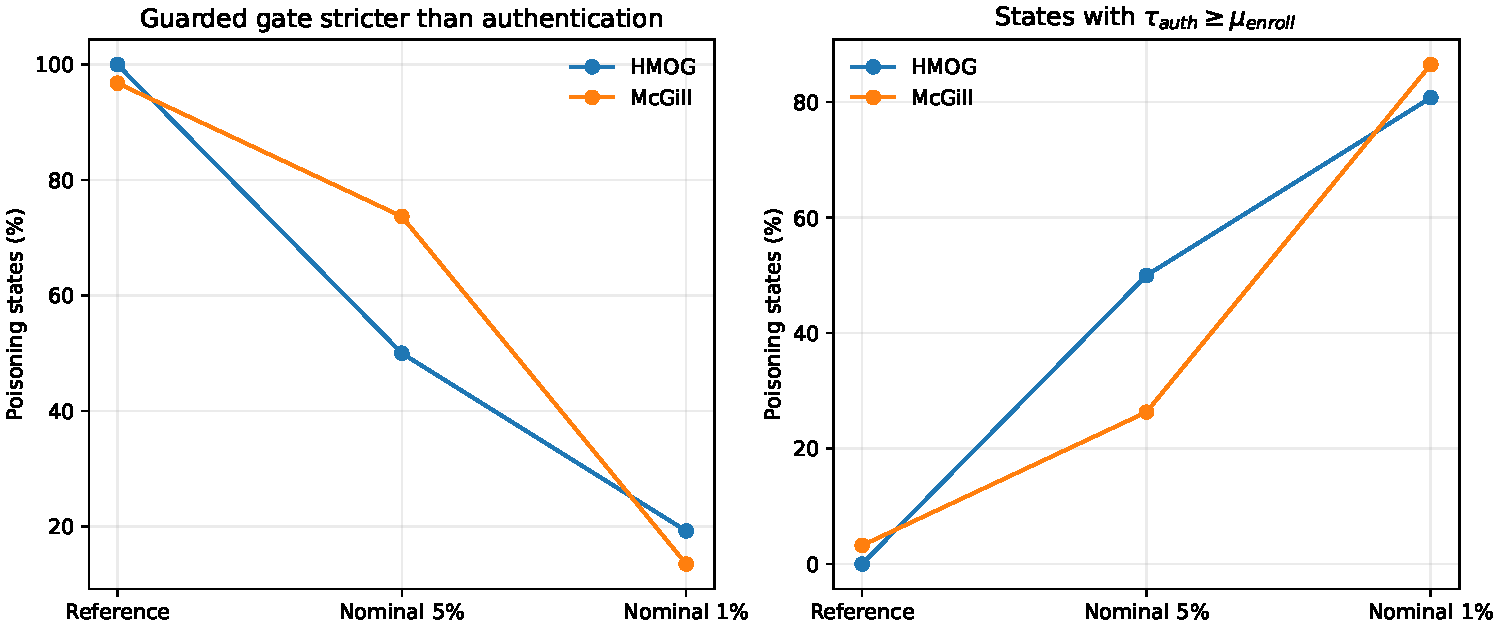
\includegraphics[width=\fulllength,height=0.72\textheight,keepaspectratio]{figures/figureS3_guarded_gate_diagnostics.pdf}
\end{adjustwidth}
\caption{Guarded gate diagnostics for boundary \(K=8\). Strict-gate and \(\tau_{\mathrm{auth}}\geq\mu_{\mathrm{enroll}}\) fractions are state-weighted over eligible poisoning states. Negative-\(k\) prevalence uses all 500 HMOG claimant-fold profiles or 20 McGill claimant profiles and is not eligibility-conditioned. Source: \protect\path{results/paper3_operating_point_sensitivity_20261004_v1/figures/guarded_gate_diagnostics.pdf}.\label{fig:s3}}
\end{figure}

\subsection*{S5. Additional HMOG temporal outcomes}\phantomsection\label{sr:s5}

Oracle-all late-FRR gains over Frozen were +4.73 points at \(D=0\) (95\% CI {[}+3.17, +6.33{]}), +5.10 at \(D=1\) ({[}+3.40, +6.80{]}), and +6.60 at \(D=2\) ({[}+4.90, +8.40{]}). Corresponding late-FAR changes were +5.51 ({[}+3.79, +7.40{]}), +5.67 ({[}+3.85, +7.71{]}), and +6.08 points ({[}+4.20, +8.16{]}). HTER gains were -0.39, -0.28, and +0.26 points; every HTER CI included zero. The \(D=0\) result shows that the Oracle contrast includes operating-point movement rather than recovery unique to synthetic shift.

\subsection*{S6. McGill frozen figures}\phantomsection\label{sr:s6}

The main article retains McGill numerical evidence in its Results and Table 3. The three frozen McGill figures are supplementary to reduce main-text duplication.

\begin{figure}[H]
\begin{adjustwidth}{-\extralength}{0cm}
\centering
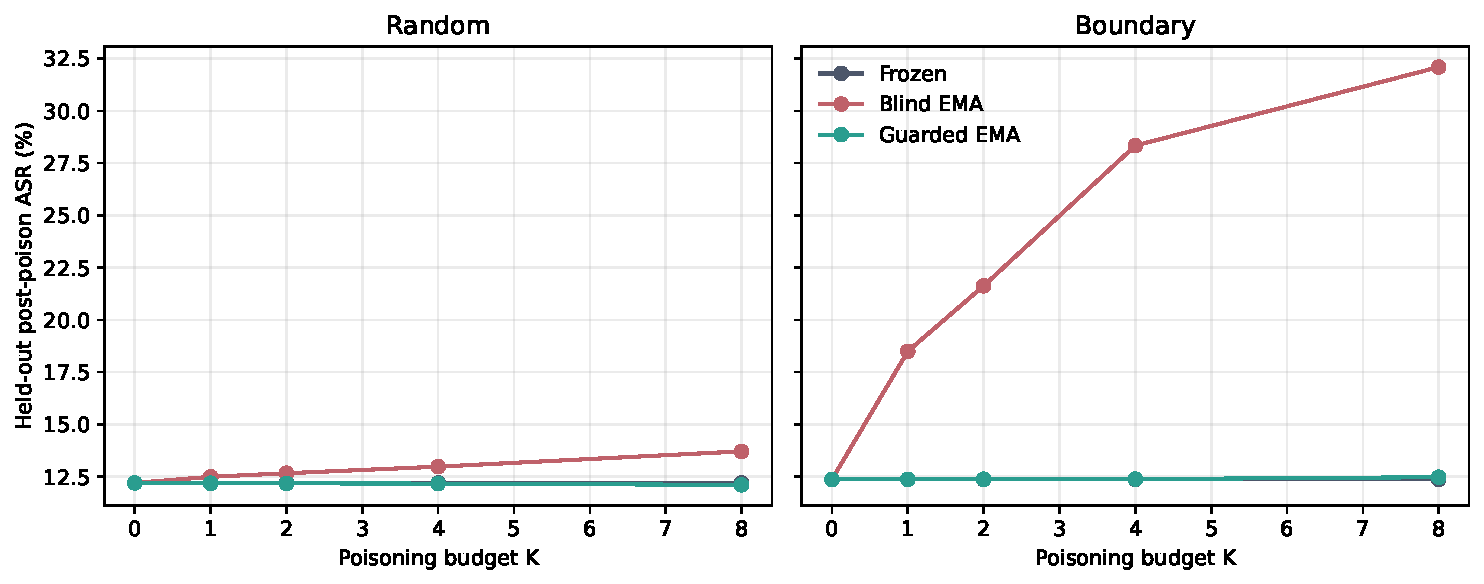
\includegraphics[width=\fulllength,height=0.72\textheight,keepaspectratio]{figures/figureS4_external_poisoning_asr.pdf}
\end{adjustwidth}
\caption{McGill reference-point post-poison ASR across nested random and score-informed boundary budgets. Poison and probe source identities are disjoint, and profiles are frozen before probe evaluation. Boundary \(K=8\) uses 1,456 eligible victim-repeat paths across 18 victims; random uses all 2,000 paths across 20 subjects. Source: \protect\path{results/paper3_external_mcgill_20261003_v1/figures/external_poisoning_asr.pdf}.\label{fig:s4}}
\end{figure}

\begin{figure}[H]
\centering
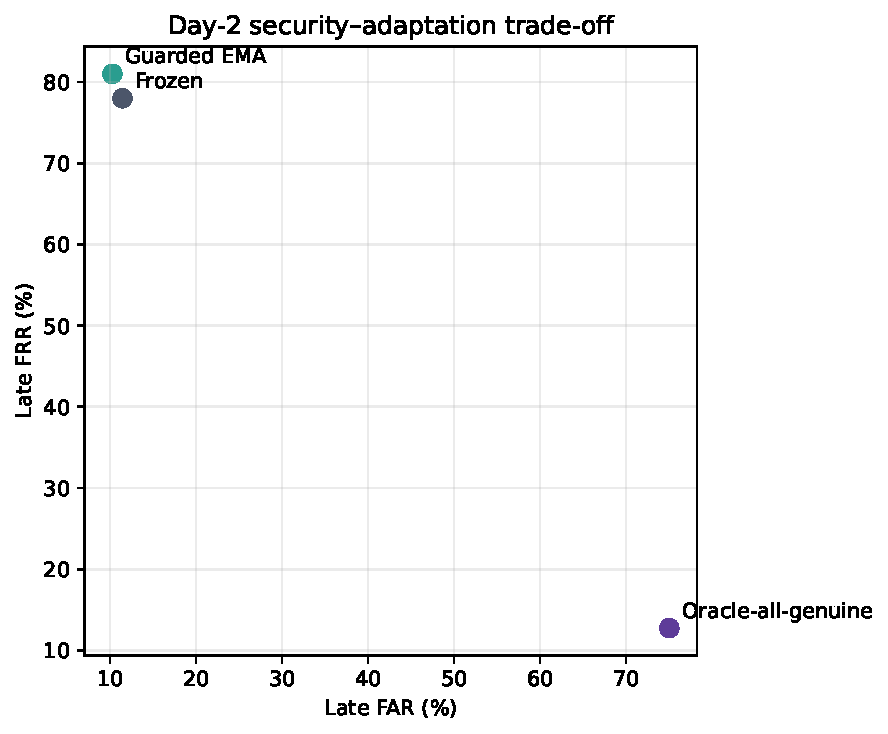
\includegraphics[width=0.92\textwidth,height=0.70\textheight,keepaspectratio]{figures/figureS5_external_temporal_tradeoff.pdf}
\caption{McGill Day-2 late FAR-FRR operating points for Frozen, Guarded EMA, and Oracle-all. Points are subject-macro estimates over the last 20 of 80 temporal units. Oracle-all is label-aware and non-deployable. Source: \protect\path{results/paper3_external_mcgill_20261003_v1/figures/external_temporal_tradeoff.pdf}.\label{fig:s5}}
\end{figure}

\begin{figure}[H]
\begin{adjustwidth}{-\extralength}{0cm}
\centering
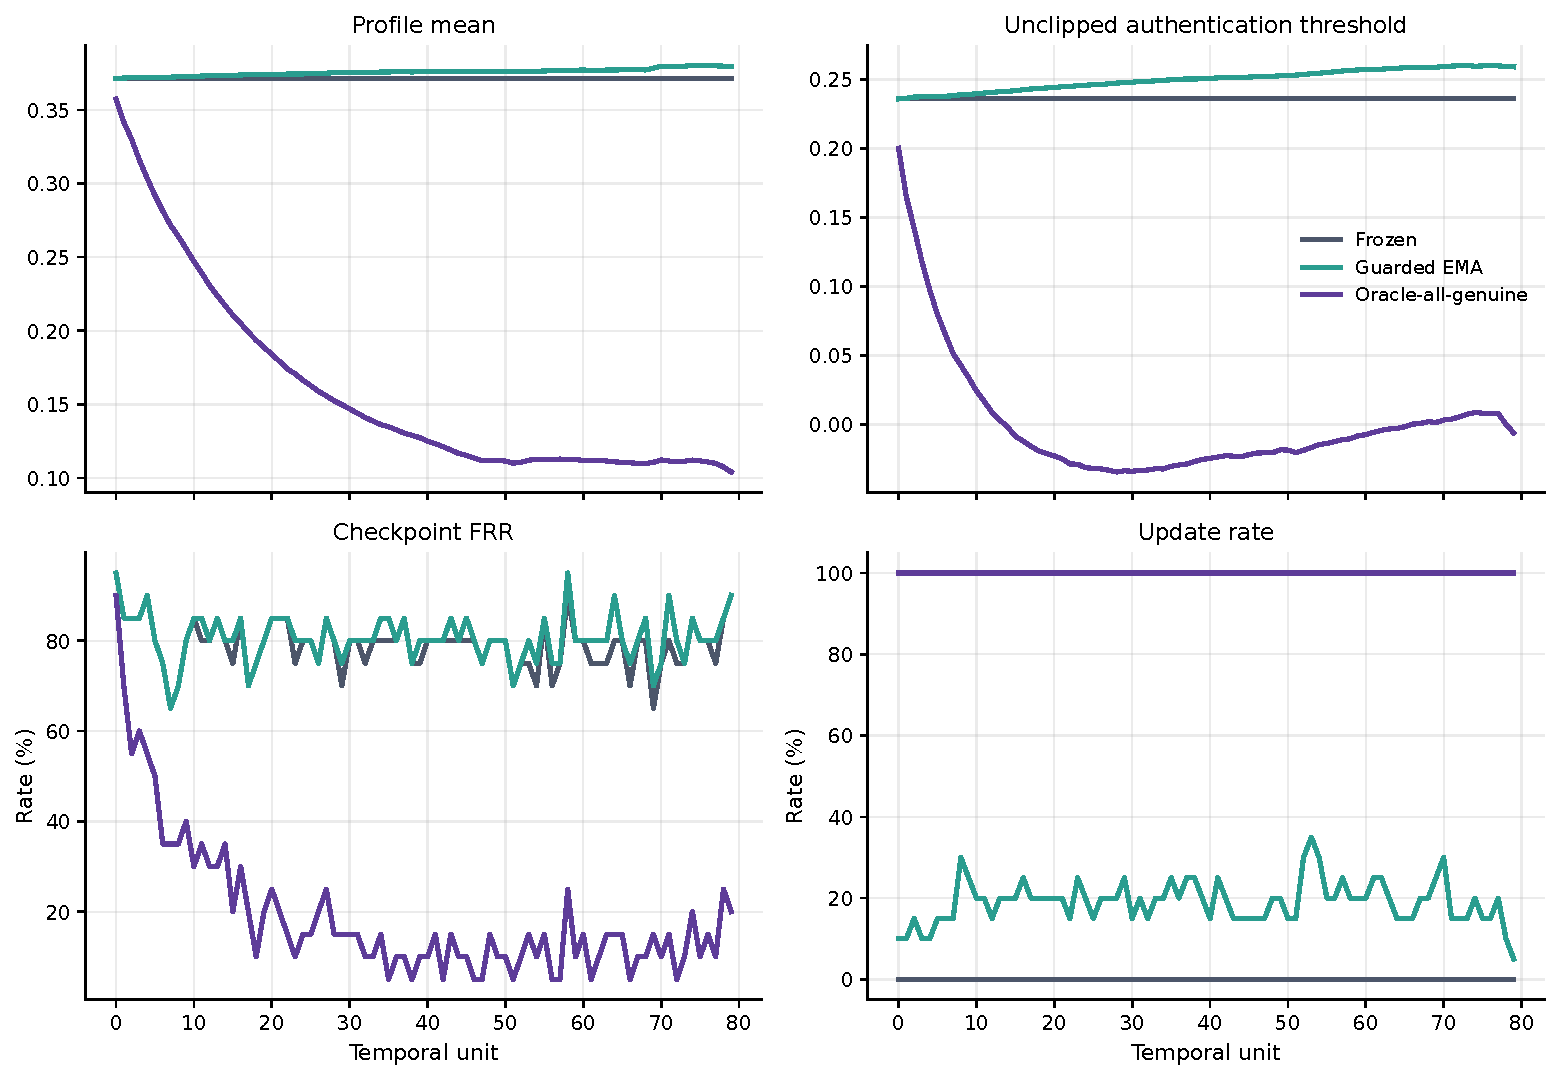
\includegraphics[width=\fulllength,height=0.72\textheight,keepaspectratio]{figures_revision_20261005/figureS6_external_selection_bias_trajectory.pdf}
\end{adjustwidth}
\caption{McGill Day-2 trajectories across 80 adaptation-checkpoint pairs. The threshold panel is the arithmetic subject-macro mean of individual \emph{unclipped authentication thresholds} \(\mu-k\sigma\), not a threshold reconstructed from aggregated moments. Authentication and update eligibility use the pre-update state; displayed profile mean, sigma-derived threshold, checkpoint FRR, and update event are saved after the adaptation step and before or at the disjoint checkpoint evaluation. All 20 subjects contribute to every unit. Negative Oracle-all thresholds are therefore executed decision thresholds, not an artwork-only raw diagnostic. Matched impostor checkpoints do not update profiles. Source: \protect\path{results/paper3_external_mcgill_20261003_v1/temporal_checkpoints.csv} and its frozen figure.\label{fig:s6}}
\end{figure}

\end{document}
